Synonims: system, application, service

% ####################### 1 PRODUCTION DATA UPLOAD ###################

\begin{table}[H]
    \centering
    \begin{tabular}[c]{|l|p{0.75\textwidth}|}
        \hline % ---------------------------------------------------------------------
    	\textsc{id}                 &   1\\
    	\hline % ---------------------------------------------------------------------
    	\textsc{Name}               &   Production data upload\\
    	\hline % ---------------------------------------------------------------------
    	\textsc{Actors}             &   Farmer\\
    	\hline % ---------------------------------------------------------------------
    	\textsc{Entry conditions}   &   Farmer has logged in\\
    	\hline % ---------------------------------------------------------------------
    	\textsc{Event flow}         &   %\footnotesize
            	                        \begin{itemize}
                                    	    \item Farmer selects the graphical element for recording production data, called informally \textit{Record Production Data button} for the sake of simplicity
                                    		\item The application displays a section that asks for more information (mandatory fields like type of production, amount of produced items, unit of measurement and optional one like description of the productivity, notes) and an element to save and upload informations, called informally \textit{Upload Button}
                                    		\item Farmer fills the mandatory fields of the current section and eventually the optional ones. Then press the Upload Button.
                                    		\item The application displays a confirm popup revealing the summary of the information is going to be recorded, asking for Farmer confirmation through a \textit{Confirm Button}
                                    		\item The farmer confirms the submission by selecting the Confirm Button
                                        \end{itemize}\\
        \hline % ---------------------------------------------------------------------
        \textsc{Exit conditions}    &  The application displays the summary page of both already uploaded product information and the previous submitted ones\\
    	\hline % ---------------------------------------------------------------------
    	\textsc{Output}             &  \begin{itemize}
    	    \item The system collects the new production data
    	    \item The farmer can visualize the list of both current production information and the previous ones
    	   % TODO (where can he visualize it?)
    	\end{itemize}\\
    	\hline % ---------------------------------------------------------------------
    	\textsc{Exceptions}         &  Farmer submits production data without filling the mandatory fields. In such case, the system displays an error message informing the Farmer about the missing field(s) required in order to achieve the goal\\
    	\hline % ---------------------------------------------------------------------
        
    \end{tabular}
    \caption{\label{tab:Production_data_submission}Use case table that describes one of the farmer functional requirements: the capability of submitting in the system his activity's usual production information.}
\end{table}


\begin{figure}[H]
	\centering
    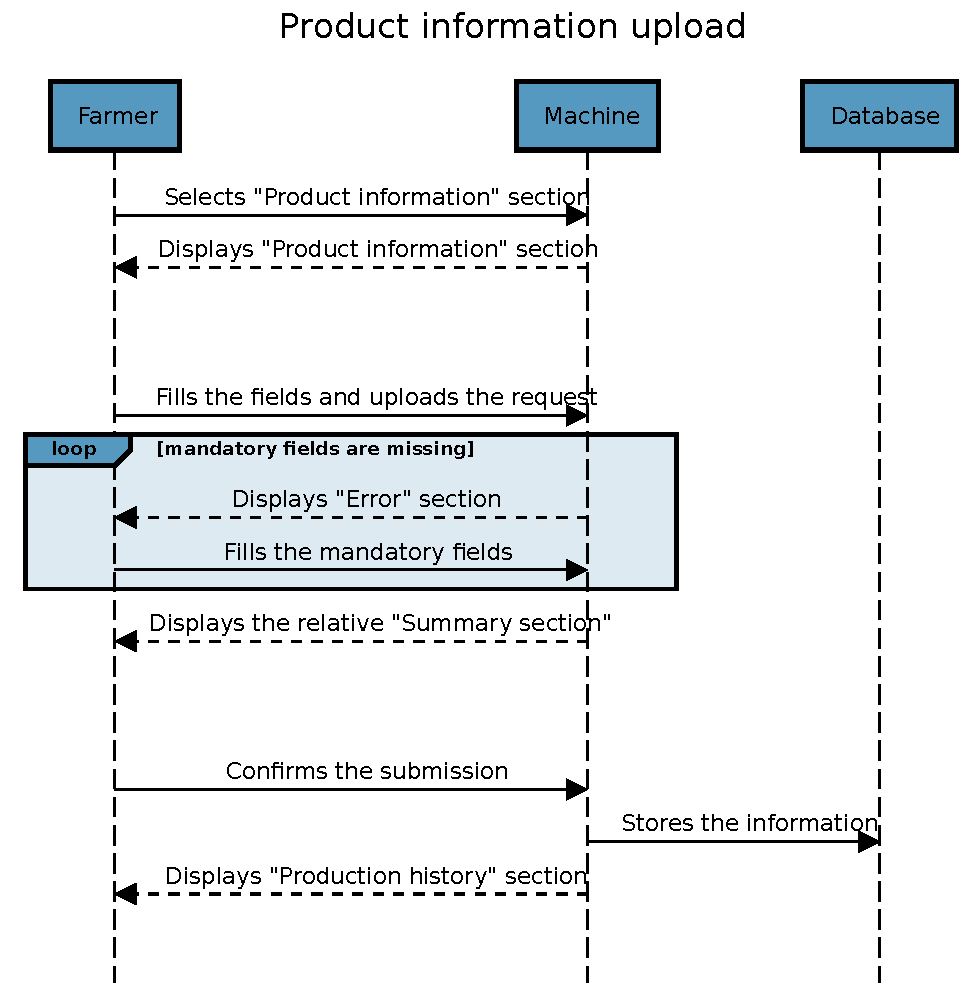
\includegraphics[page=1, width=\textwidth]{Images/SeqDiag/product_info_upload_seq_diag.pdf}
	\caption{\label{fig:product_info_seq_diag}High level UML sequence diagram of the production data submission process}
\end{figure}


% ####################### 2 SUGGESTION REQUEST ###################

\begin{table}[H]
    \centering
    \begin{tabular}{|l|p{0.75\textwidth}|}
        \hline % ---------------------------------------------------------------------
    	\textsc{id}                 &   2\\
    	\hline % ---------------------------------------------------------------------
    	\textsc{Name}               &   Help/suggestion request\\
    	\hline % ---------------------------------------------------------------------
    	\textsc{Actors}             &   Farmer\\
    	\hline % ---------------------------------------------------------------------
    	\textsc{Entry conditions}   &   Farmer has logged in\\
    	\hline % ---------------------------------------------------------------------
    	\textsc{Event flow}         &   %\footnotesize
            	                        \begin{itemize}
                                    	    \item Farmer selects the graphical section responsible of the private requests, called informally \textit{request section} for the sake of simplicity
                                    		\item The application displays a section that presents an eventual list of previous request chats, and an internal element to send a new private request, called informally \textit{Send request element}
                                    		\item Farmer selects the send request button
                                    		\item The application displays a new section that present all the Farmer's saved contacts
                                    		\item The farmer selects the contact he wants to send the request
                                    		\item The system displays a section with an editable text form and a send button.
                                    		\item The farmer writes the request and selects the send button
                                        \end{itemize}\\
        \hline % ---------------------------------------------------------------------
        \textsc{Exit conditions}    &  The application displays the summary page of both already sent request chat and the previous submitted ones\\
    	\hline % ---------------------------------------------------------------------
    	\textsc{Output}             &  \begin{itemize}
    	    \item The system collects the new request chat
    	    \item The farmer can visualize the list of both current request chat and the previous ones
    	   % TODO (where can he visualize it?)
    	\end{itemize}\\
    	\hline % ---------------------------------------------------------------------
    	\textsc{Exceptions}         &  Farmer selects the request button without editing the text form. In such case, the system displays an error message informing the Farmer about the missing field required in order to achieve the goal\\
    	\hline % ---------------------------------------------------------------------
        
    \end{tabular}
    \caption{\label{tab:Help_request_submission}Use case table that describes one of the farmer functional requirements: the capability of submitting in the system help requests to other farmers and/or agronomists in a private way.}

\end{table}

\begin{figure}[H]
	\centering
    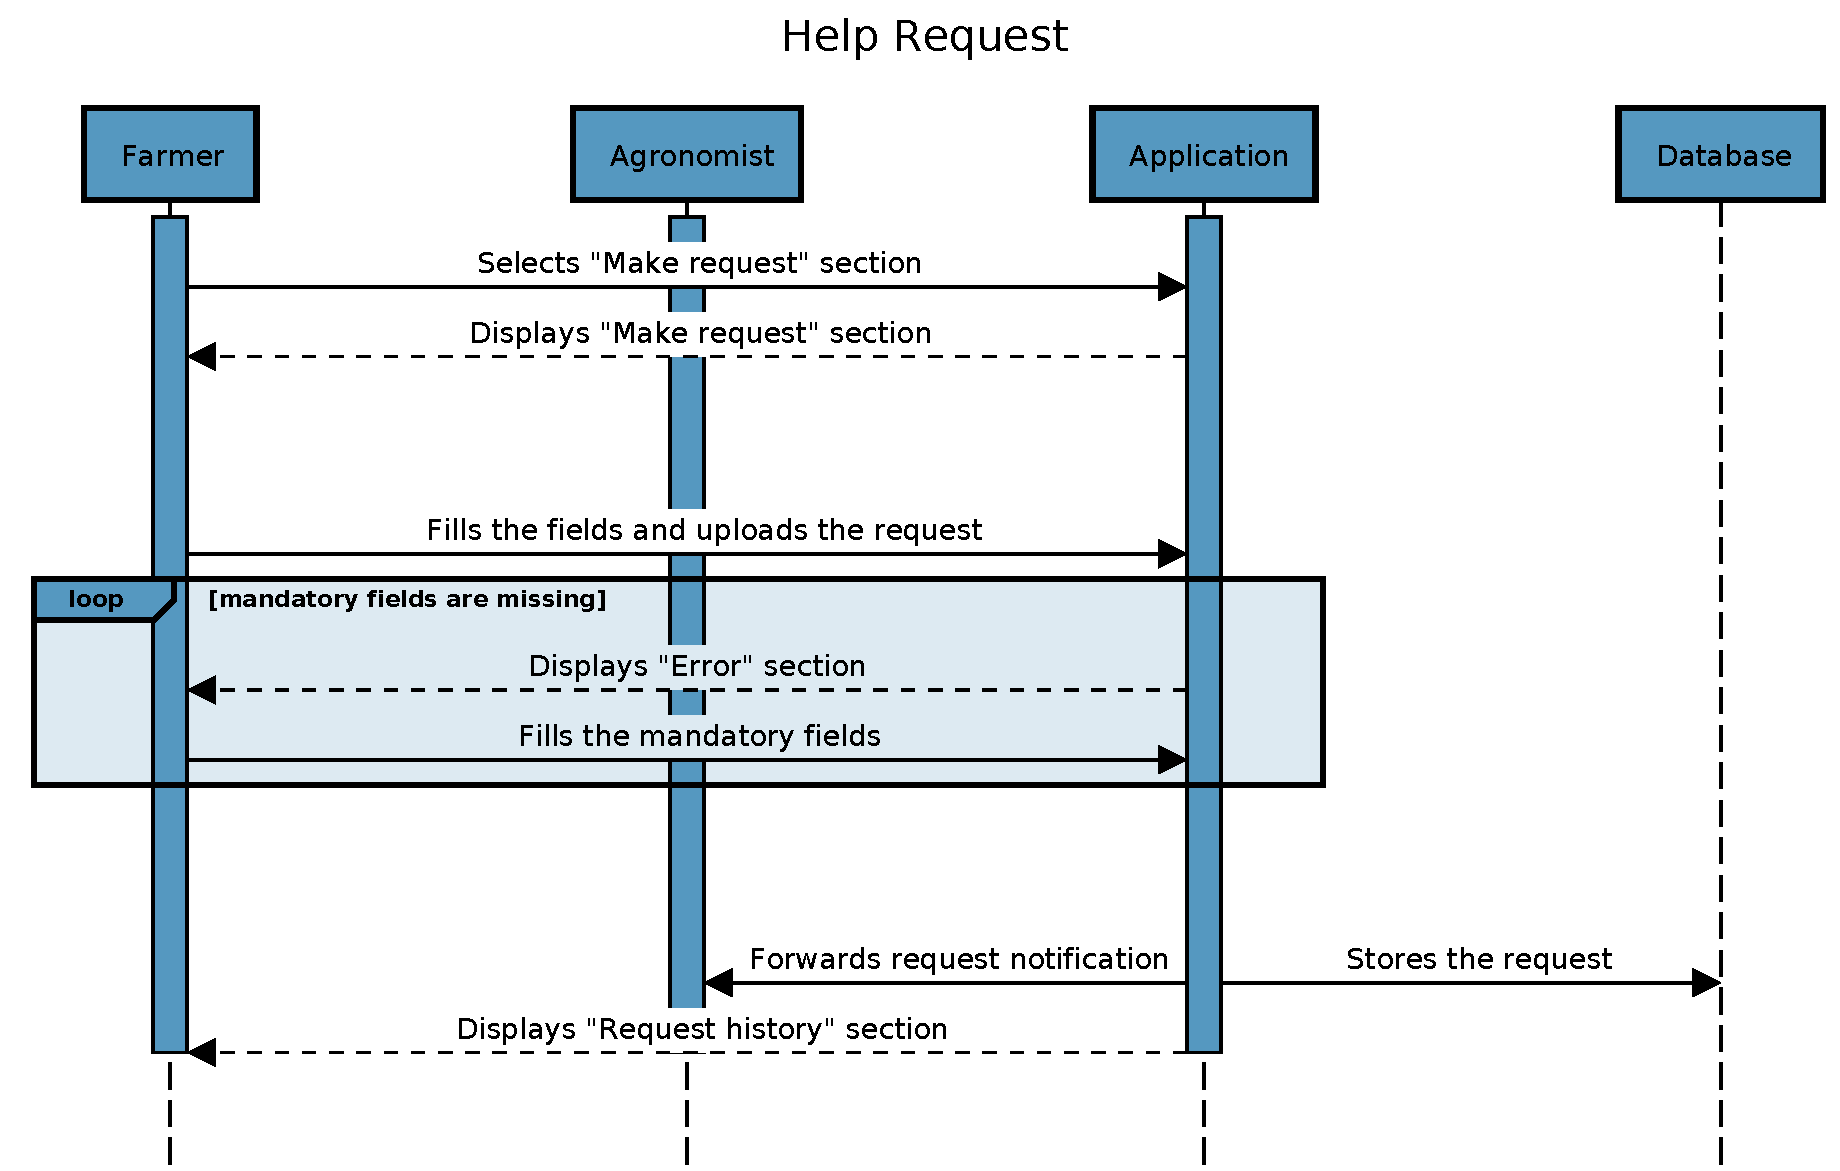
\includegraphics[page=1, width=\textwidth]{Images/SeqDiag/help_request_seq_diag.pdf}
	\caption{\label{fig:help_request_seq_diag}High level UML sequence diagram of the help request process}
\end{figure}

% ####################### 3 FORUM GENERATION ###################

\begin{table}[H]
    \centering
    \begin{tabular}{|l|p{0.75\textwidth}|}
        \hline % ---------------------------------------------------------------------
    	\textsc{id}                 &   3\\
    	\hline % ---------------------------------------------------------------------
    	\textsc{Name}               &   Forum generation\\
    	\hline % ---------------------------------------------------------------------
    	\textsc{Actors}             &   Farmer\\
    	\hline % ---------------------------------------------------------------------
    	\textsc{Entry conditions}   &   Farmer has logged in\\
    	\hline % ---------------------------------------------------------------------
    	\textsc{Event flow}         &   %\footnotesize
            	                        \begin{itemize}
                                    	    \item Farmer selects the graphical section responsible of the forum generation, called informally \textit{Forum section} for the sake of simplicity
                                    		\item The application displays a section that presents an eventual list that contains both previous submitted forums and farmer's forum replies, and an internal element to submit a new public forum, called informally \textit{forum upload button}
                                    		\item Farmer selects the forum upload button
                                    		\item The application displays a new section that present 3 mandatory fields (the topic/context of the thread, the title and the question content) and a submission button
                                    		\item The farmer fills all the mandatory fields and selects the submission button
                                    		\item The application displays a confirm popup revealing the summary of the information is going to be uploaded, asking for Farmer confirmation through a \textit{Confirm Button}
                                    		\item The farmer confirms the submission by selecting the Confirm Button
                                        \end{itemize}\\
        \hline % ---------------------------------------------------------------------
        \textsc{Exit conditions}    &  The application displays the summary page containing both already submitted forum thread, the previous submitted ones and the ones whose the farmer replied\\
    	\hline % ---------------------------------------------------------------------
    	\textsc{Output}             &  \begin{itemize}
    	    \item The system collects the new forum thread
    	    \item The farmer can visualize the list containing both current forum thread, the previous submitted ones and the ones whose the farmer replied
    	   % TODO (where can he visualize it?)
    	\end{itemize}\\
    	\hline % ---------------------------------------------------------------------
    	\textsc{Exceptions}         &   Farmer submits Forum thread without filling all the mandatory fields. In such case, the system displays an error message informing the Farmer about the missing field(s) required in order to achieve the goal\\
    	\hline % ---------------------------------------------------------------------
        
    \end{tabular}

\caption{\label{tab:Forum_generation}Use case table that describes one of the farmer functional requirements: the capability of submitting in the system public forum threads}
\end{table}

\begin{figure}[H]
	\centering
    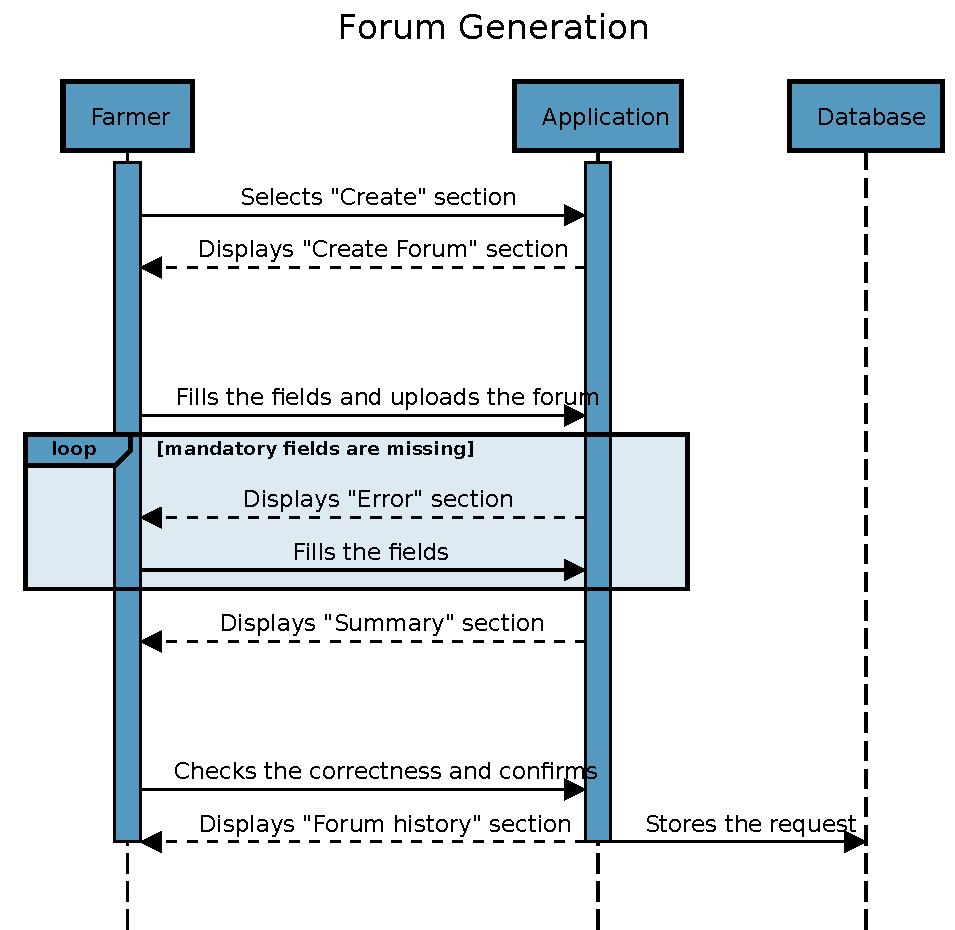
\includegraphics[page=1, width=\textwidth]{Images/SeqDiag/forum_generation_seq_diag.pdf}
	\caption{\label{fig:forum_generation_seq_diag}High level UML sequence diagram of the forum generation process}
\end{figure}

% ####################### 4 PROBLEM INFORMATION ###################


\begin{table}[H]
    \centering
    \begin{tabular}{|l|p{0.75\textwidth}|}
        \hline % ---------------------------------------------------------------------
    	\textsc{id}                 &   4\\
    	\hline % ---------------------------------------------------------------------
    	\textsc{Name}               &   Problem information upload\\
    	\hline % ---------------------------------------------------------------------
    	\textsc{Actors}             &   Farmer\\
    	\hline % ---------------------------------------------------------------------
    	\textsc{Entry conditions}   &   Farmer has logged in\\
    	\hline % ---------------------------------------------------------------------
    	\textsc{Event flow}         &   %\footnotesize
            	                        \begin{itemize}
                                    	    \item Farmer selects the graphical section responsible for the problem information submission, called informally \textit{Problems section}
                                    		\item The application displays a section that requires for information (described previously) and a "submit button"
                                    		\item Farmer fills the mandatory fields and eventually the optional ones, then selects the upload button
                                    		\item The application displays a confirm popup revealing the summary of the information is going to be uploaded, asking for Farmer confirmation through a \textit{Confirm Button}
                                    		\item The farmer confirms the submission by selecting the Confirm Button
                                        \end{itemize}\\
        \hline % ---------------------------------------------------------------------
        \textsc{Exit conditions}    &  The application displays the summary page containing both already submitted problem information and the previous submitted ones\\
    	\hline % ---------------------------------------------------------------------
    	\textsc{Output}             &  \begin{itemize}
    	    \item The system collects the new problem information instance
    	    \item The farmer can visualize the list containing both the current submitted problem information and the previous submitted ones
    	   % TODO (where can he visualize it?)
    	\end{itemize}\\
    	\hline % ---------------------------------------------------------------------
    	\textsc{Exceptions}         &   Farmer submits problem information without filling all the mandatory fields. In such case, the system displays an error message informing the Farmer about the missing field(s) required in order to achieve the goal\\
    	\hline % ---------------------------------------------------------------------
        
    \end{tabular}

\caption{\label{tab:problem_information}Use case table that describes one of the farmer functional requirements: the capability of submitting in the system problem information}
\end{table}

% ####################### 5 GOOD PRACTICES ###################

\begin{table}[H]
    \centering
    \begin{tabular}{|l|p{0.75\textwidth}|}
        \hline % ---------------------------------------------------------------------
    	\textsc{id}                 &   5\\
    	\hline % ---------------------------------------------------------------------
    	\textsc{Name}               &   Good practices upload\\
    	\hline % ---------------------------------------------------------------------
    	\textsc{Actors}             &   Farmer\\
    	\hline % ---------------------------------------------------------------------
    	\textsc{Entry conditions}   &   Farmer has logged in\\
    	\hline % ---------------------------------------------------------------------
    	\textsc{Event flow}         &   %\footnotesize
            	                        \begin{itemize}
                                    	    \item Farmer selects the graphical section responsible for the good practices document submission, called informally \textit{document section}
                                    		\item The application displays a section that requires for information (described previously) and a "submit button"
                                    		\item Farmer fills the mandatory fields and eventually the optional ones, then selects the upload button
                                    		\item The farmer confirms the submission by selecting the Confirm Button
                                        \end{itemize}\\
        \hline % ---------------------------------------------------------------------
        \textsc{Exit conditions}    &  The application displays the summary page containing both already submitted document and the previous submitted ones\\
    	\hline % ---------------------------------------------------------------------
    	\textsc{Output}             &  \begin{itemize}
    	    \item The system collects the new document
    	    \item The farmer can visualize the list containing both the current submitted document and the previous submitted ones
    	   % TODO (where can he visualize it?)
    	\end{itemize}\\
    	\hline % ---------------------------------------------------------------------
    	\textsc{Exceptions}         &   Farmer submits document without filling all the mandatory fields. In such case, the system displays an error message informing the Farmer about the missing field(s) required in order to achieve the goal\\
    	\hline % ---------------------------------------------------------------------
        
    \end{tabular}

\caption{\label{tab:good_practice_submission}Use case table that describes one of the farmer functional requirements: the capability of submitting in the system good practices document}
\end{table}

\begin{figure}[H]
	\centering
    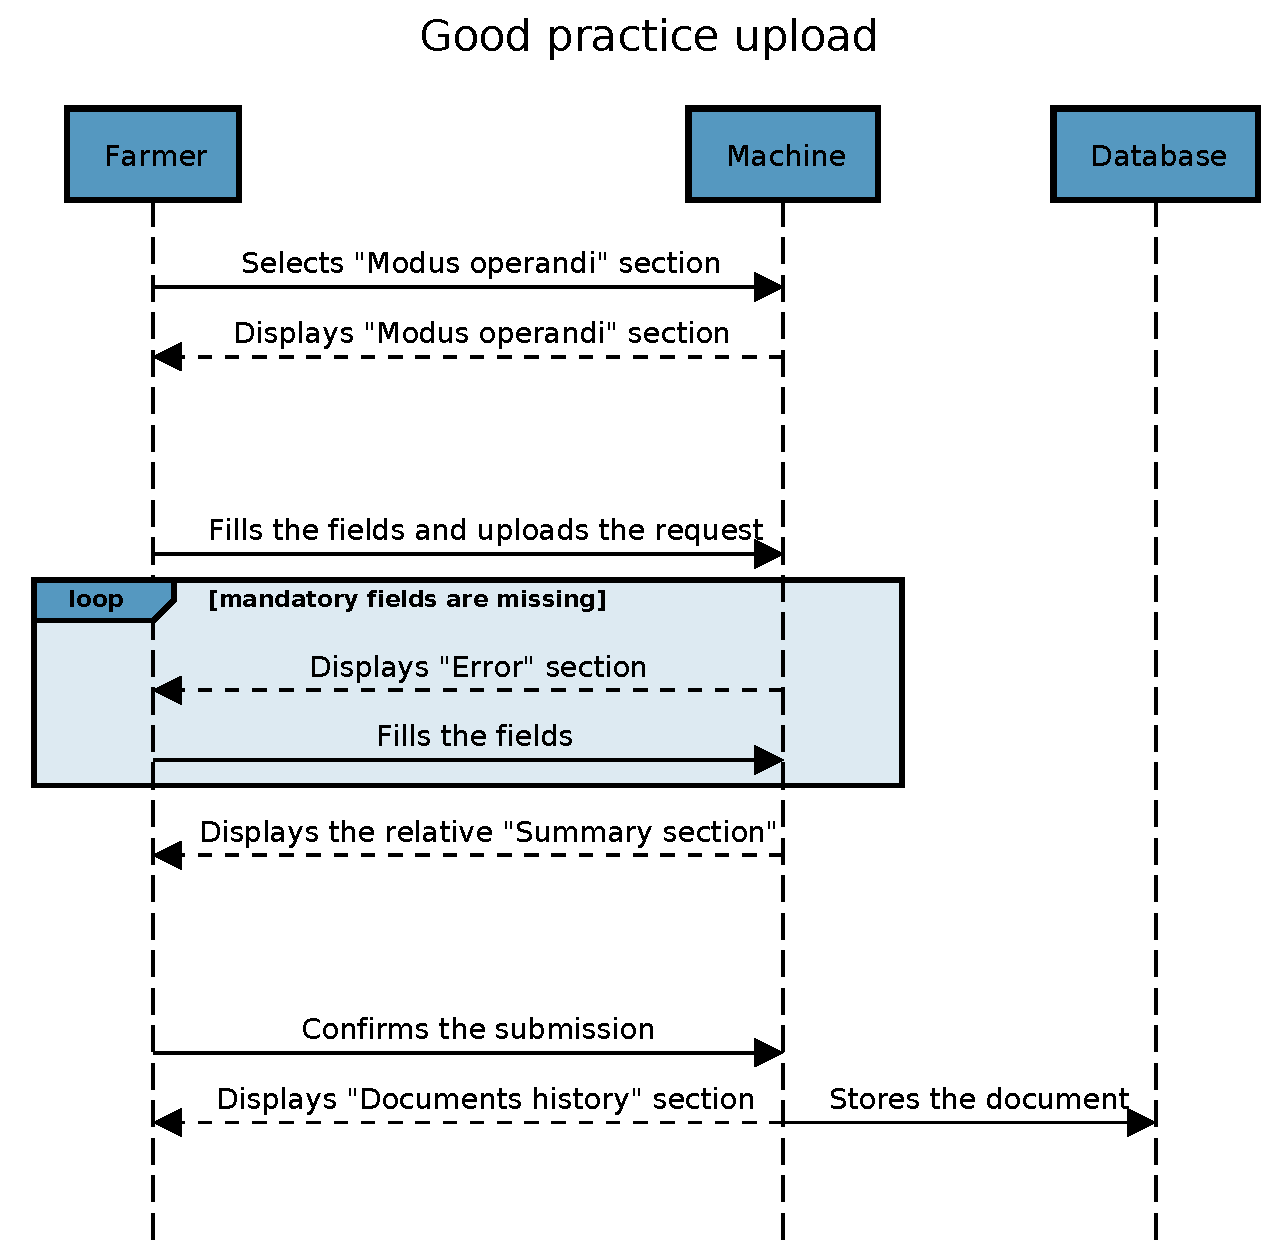
\includegraphics[page=1, width=\textwidth]{Images/SeqDiag/good_practice_seq_diag.pdf}
	\caption{\label{fig:good_practice_seq_diag}High level UML sequence diagram of the good practices document submission process}
\end{figure}


\begin{table}[H]
    \centering
    \begin{tabular}{|l|p{0.75\textwidth}|}
        \hline % ---------------------------------------------------------------------
    	\textsc{id}                 &   6\\
    	\hline % ---------------------------------------------------------------------
    	\textsc{Name}               &   Visualize relevant data\\
    	\hline % ---------------------------------------------------------------------
    	\textsc{Actors}             &   Farmer\\
    	\hline % ---------------------------------------------------------------------
    	\textsc{Entry conditions}   &   Farmer has logged in\\
    	\hline % ---------------------------------------------------------------------
    	\textsc{Event flow}         &   %\footnotesize
            	                        \begin{itemize}
                                    	    \item Farmer selects the graphical section responsible for the relevant data visualization, called informally \textit{Relevant section}
                                        \end{itemize}\\
        \hline % ---------------------------------------------------------------------
        \textsc{Exit conditions}    &  The application displays a section containing information about weather forecasts, farm related tools suggestion, agronomist visit time, amount of water used that month, soil humidity etc.)\\
    	\hline % ---------------------------------------------------------------------
    	\textsc{Output}             &  \begin{itemize}
    	    \item The farmer can visualize relevant informations
    	    \item Farmer can interact with information (links to shop websites etc.)
    	   % TODO (where can he visualize it?)
    	\end{itemize}\\
    	\hline % ---------------------------------------------------------------------
    	\textsc{Exceptions}         &   If the internet connection is lost, the application displays a section informing the task cannot be achieved\\
    	\hline % ---------------------------------------------------------------------
        
    \end{tabular}

\caption{\label{tab:visualize_relevant_data}Use case table that describes one of the farmer goals: visualize relevant data}
\end{table}